\documentclass[paper=a4]{article}
\usepackage{ucs}
\usepackage[utf8x]{inputenc}
\usepackage[T1]{fontenc}
\PreloadUnicodePage{0}
\usepackage{xspace}
\usepackage{array}
\usepackage[hmargin=3.5cm,vmargin=2.7cm]{geometry} 
\usepackage{graphicx}


\title{Spillmanual}
\author{Team Dank}
\begin{document}
\maketitle

\section{Introduksjon}
Dette er et spill tiltenkt datamaskiner der spilleren kjører en bil.
Bilen kjører langs en vei med forskjellige ting i veibanen, som spilleren kan kjøre over eller unngå.
Vanndammer vil gjøre at spilleren mister drivstoff, og mister litt kontrollen over bilen.
Kumlokk i veien gjør at spilleren taper.
Bensintanker gir spilleren ekstra drivstoff, slik at runden varer lenger.
Myke trafikanter vil gi poeng til spilleren dersom de blir påkjørt.
Mynter kan plukkes opp slik at spilleren kan kjøpe nye biler.
Spilleren får en score for hver spillrunde, i tillegg til at spilleren samler opp virtuelle penger som kan brukes til å bytte bil.
\begin{center}
\begin{tabular}{ | m{5cm} | m{8cm} | }
\hline
Målgruppe. & Ungdom 15-25 år. \\ \hline
Spillvarighet. & Spillet varer helt til bilen går tom for bensin eller til spilleren kjører på at kumlokk.\\&
Dette kan ta alt fra få sekunder til mange minutter, da spiller kan plukke opp mer bensin på veien, eller kræsje med en gang.\\ \hline
Spillere. & En-spiller spill. \\ \hline
Åpne data. & Bruke åpne data fra yr.no om været. Om det er skyer vil det være skyer på banen,\\&
om det regner vil det regne på banen, og om det snør vil det være snø på banen.\\ \hline
\end{tabular}
\end{center}

\begin{center}
\begin{tabular}{ | m{4cm} | m{10cm}|} 
\hline
Pre-condition & 
Spillet er startet \\&
\\ \hline

Standard path & 
S01 Bruker står i starmenyen \\&
S02 Trykker `play` \\&
S03 Spillet starter \\&
S04 Bruker holder inne til høyre eller venstre for å styre \\&
S05 Bruker unngår hindringene \\&
S06 Bruker plukker opp myntene\\&
S07 Bruker plukker opp bensintankene dersom det kommer\\&
S08 Bruker spiller til tom for bensin \\&
S09 Spillet stopper \\&
S10 Spillet viser high-score og ekstra penger \\&
S11 Spillet lagrer \\&
S12 Spillet går tilbake til startskjermen \\&
\\ \hline

Post-condition & 
Spillet er klar til å avsluttes eller starte på nytt \\&
\\ \hline

Alternative Path & 
A01: @S01, Bruker kan trykke på oppgrader knappen\\& 
		A01.01 Bruker kjøper oppgraderinger dersom han vil\\&
		A01.02 Bilen i spillet blir bedre \\&
		A01.03 Bruker trykker på tilbake-knappen \\&
		A01.04 RESUME @S01 \\&
		\\&
A02: @S01, Bruker kan trykke på tannhjul knappen\\& 
		A02.01 Bruker endrer på instillingene han vil\\&
		A02.02 Spillet godtar instillingene \\&
		A01.03 Bruker trykker på tilbake-knappen \\&
		A02.04 RESUME @S01 \\&
		\\&
A03: @S04-07, Bruker kan når som helst trykke på pause mens han spiller spillet\\&
		A03.01 Spillet settes på pause \\& 
		A03.02 Bruker kan trykke `Avslutt` eller `Fortsett`\\& 
		A03.03 Dersom bruker trykker på `Avslutt`\\& 
		A03.04 RESUME @S09 \\&
		
\\ \hline
\end{tabular}
Use-case: Spille spillet
\end{center}

	\section{Spillregler}
		\subsection{Kontroll}
		\begin{itemize}
			\item{Spilleren kan styre bilen til høyre og venstre ved hjelp av piltastene eller A og D.}
			\item{Spilleren kan ikke styre bilens hastighet direkte.}
			\item{Bilen kan ikke styres av veien.}
			\item{Man går til pausemenyen ved å trykke på ESC.}
		\end{itemize}

		\subsection{Objektinteraksjon}
		\begin{itemize}
			\item{Bilen kan treffe objekter i veien.}
			\item{Objekter kan påføre bilen en positiv, eller negativ effekt.}
			\item{Mynter vil gi spilleren mulighet til å kjøpe nye biler.}
			\item{Bensintanker vil gi spilleren mer drivstoff, slik at spillet varer lengre.}
			\item{Myke trafikanter vil gi spilleren mer poeng dersom de blir påkjørt.}
			\item{Vanndammer vil minske mengden drivstoff, og samtidig gjøre at spilleren mister litt kontrollen av bilen.}
			\item{Kumlokk vil avslutte spillet.}
		\end{itemize}

		\subsection{Poeng}
		\begin{itemize}
			\item{Spilleren tjener poeng konstant når han kjører.}
			\item{Poeng blir opptjent avhengig av hvor langt spilleren kjører og hvilke myke trafikanter spilleren kjører over.}
			\item{Spilleren starter alltid med 0 poeng i starten av en runde.}
		\end{itemize}

		\subsection{Penger}
		\begin{itemize}
			\item{I løpet av spillet får spilleren penger i form av spillets egen valuta.}
			\item{Pengene kan brukes i spillets butikk fra hovedmenyen for å kjøpe nye biler.}
		\end{itemize}

	\section{Brukerhistorier}
		\begin{itemize}
			\item{Som spiller vil jeg ha mulighet til å styre bilen for å kunne velge hva jeg vil kjøre over.}
			\item{Som spiller vil jeg ha mulighet til å sette spillet på pause når jeg vil for å kunne gjøre andre ting.}
			\item{Som spiller vil jeg ha mulighet til å avslutte spiller når jeg vil i tilfelle jeg ikke har tid til å spille mer.}
			\item{Som spiller vil jeg ha mulighet til å oppgradere bilen min for å få en følelse av progressjon.}
			\item{Som spiller vil jeg ha mulighet til å se mine høyeste poengscore for å kunne måle min egen progressjon i spillet.}
			\item{Som spiller vil jeg ha mulighet til å justere lydvolumet på spillet for å ikke vere forstyrrende på bussen.}
		\end{itemize}

	\newpage
	\begin{figure}\begin{center}
		
\includegraphics[width=1.00\textwidth]{images/main_menu.PNG}
		\caption{Hovedmeny.}
	\end{center}\end{figure}

	\begin{figure}\begin{center}
		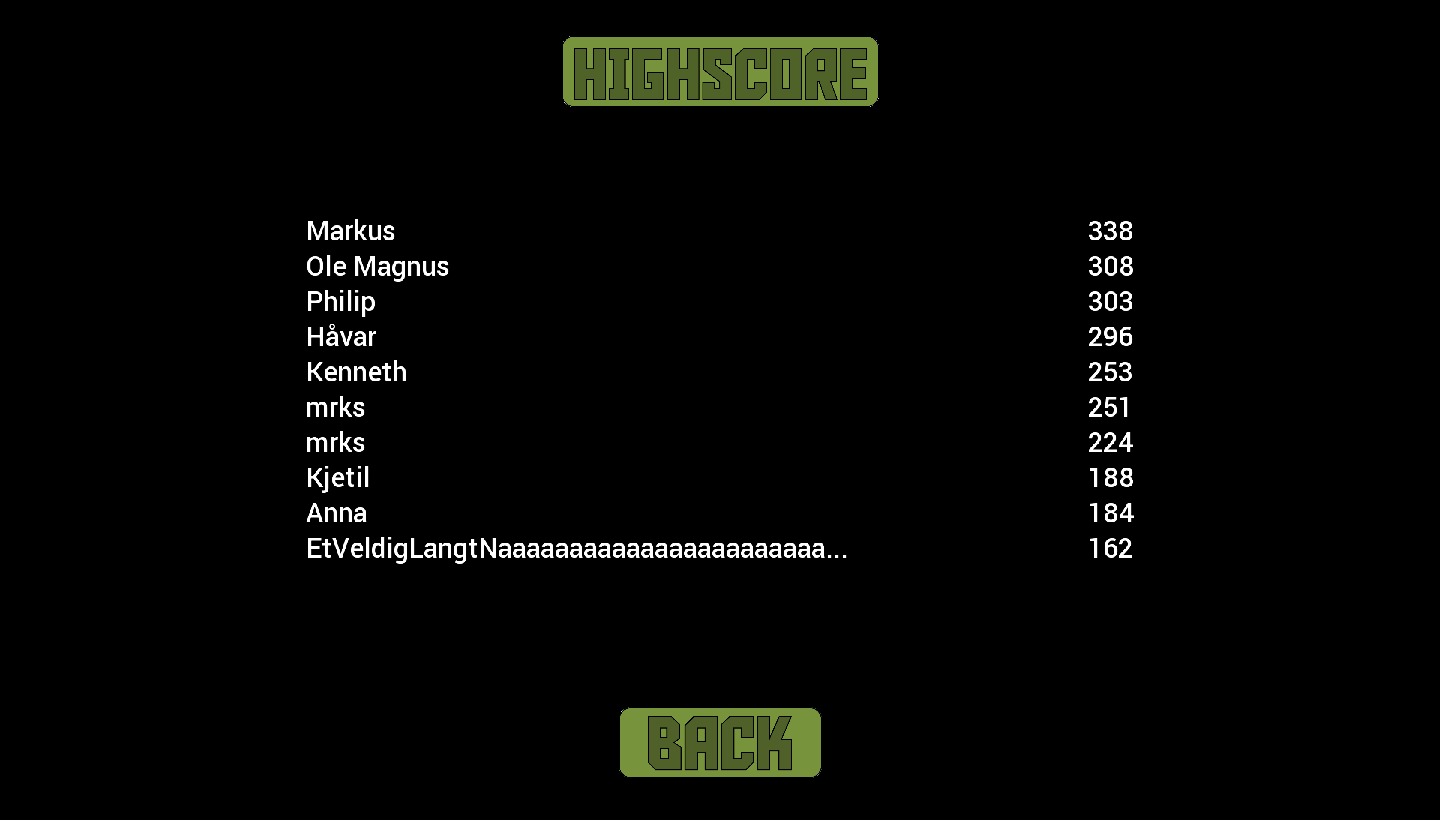
\includegraphics[width=1.00\textwidth]{images/hs_menu.PNG}
		\caption{Highscoremeny.}
	\end{center}\end{figure}

	\begin{figure}\begin{center}
		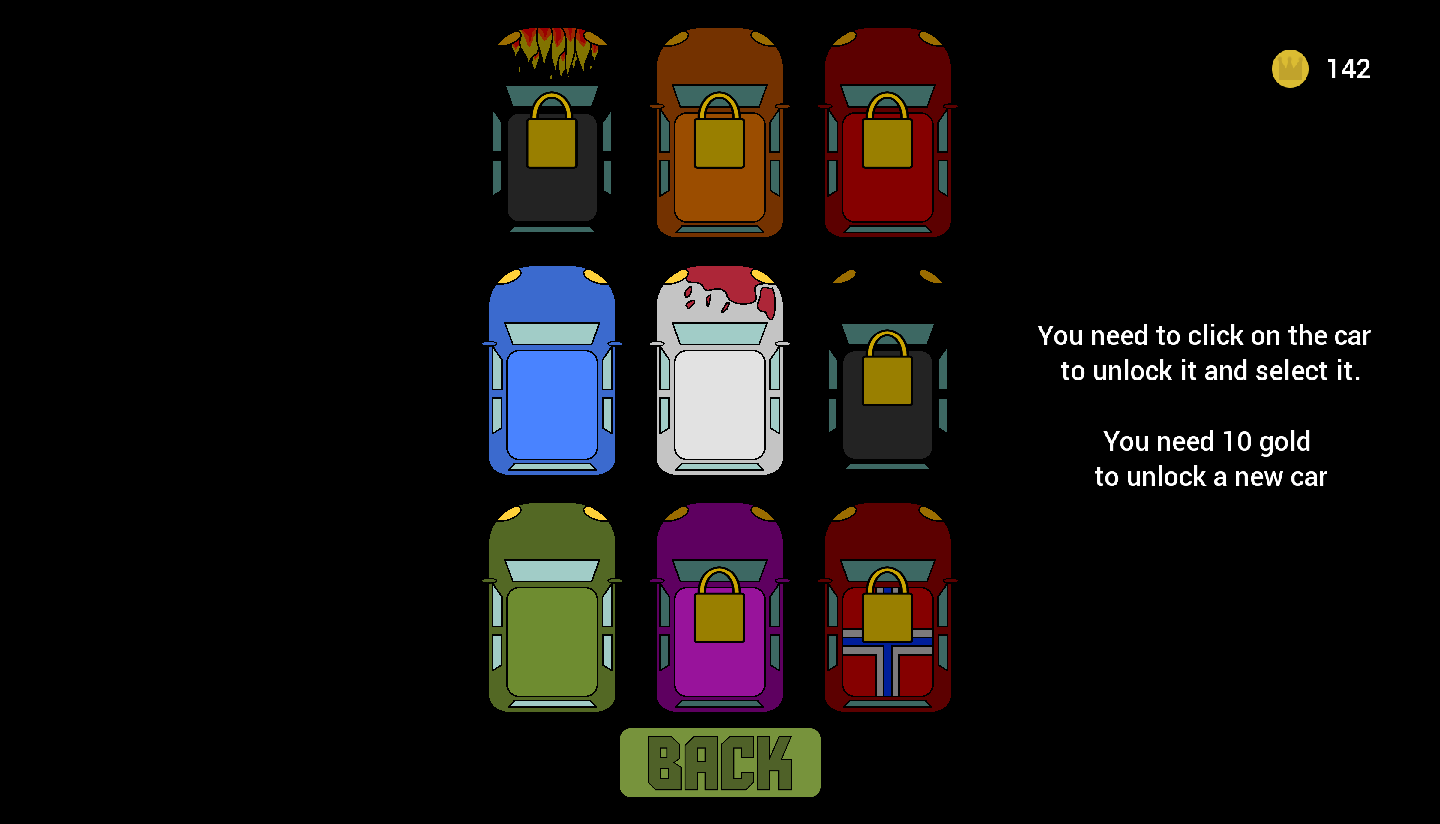
\includegraphics[width=1.00\textwidth]{images/shop_menu.PNG}
		\caption{Butikkmeny.}
	\end{center}\end{figure}

	\begin{figure}\begin{center}
		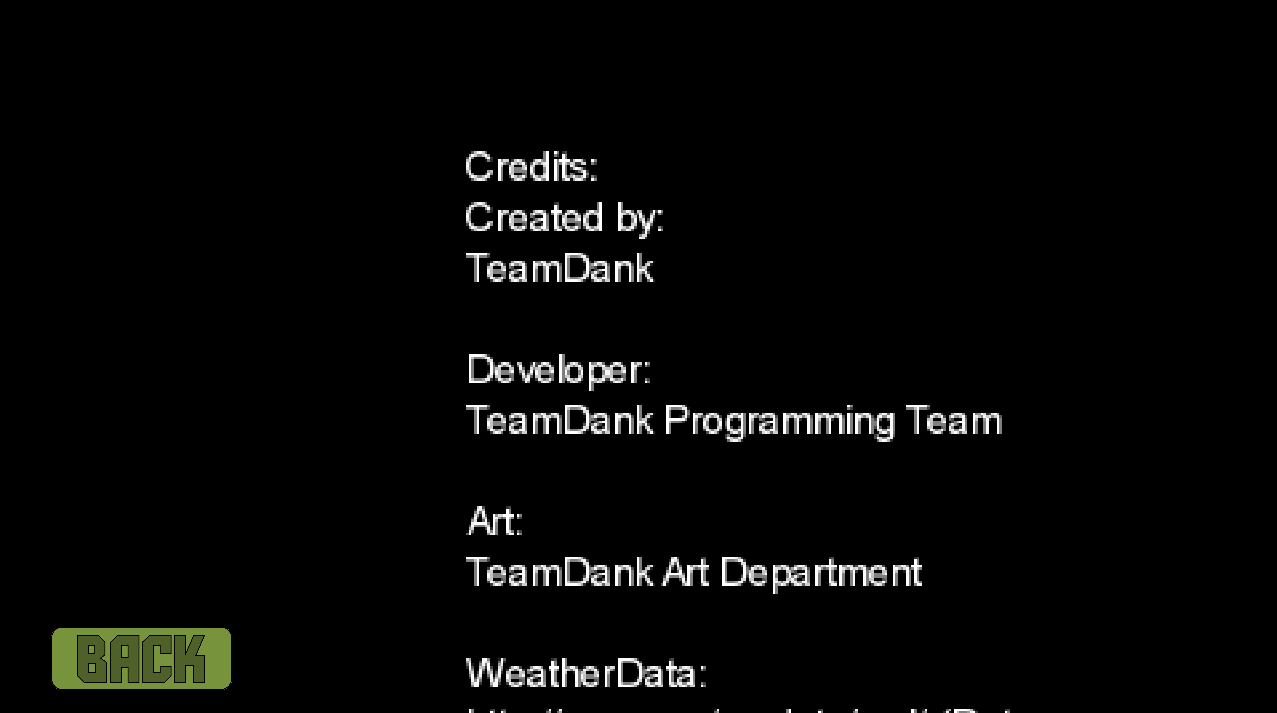
\includegraphics[width=1.00\textwidth]{images/credits.PNG}
		\caption{Kreditering.}
	\end{center}\end{figure}

	\begin{figure}\begin{center}
		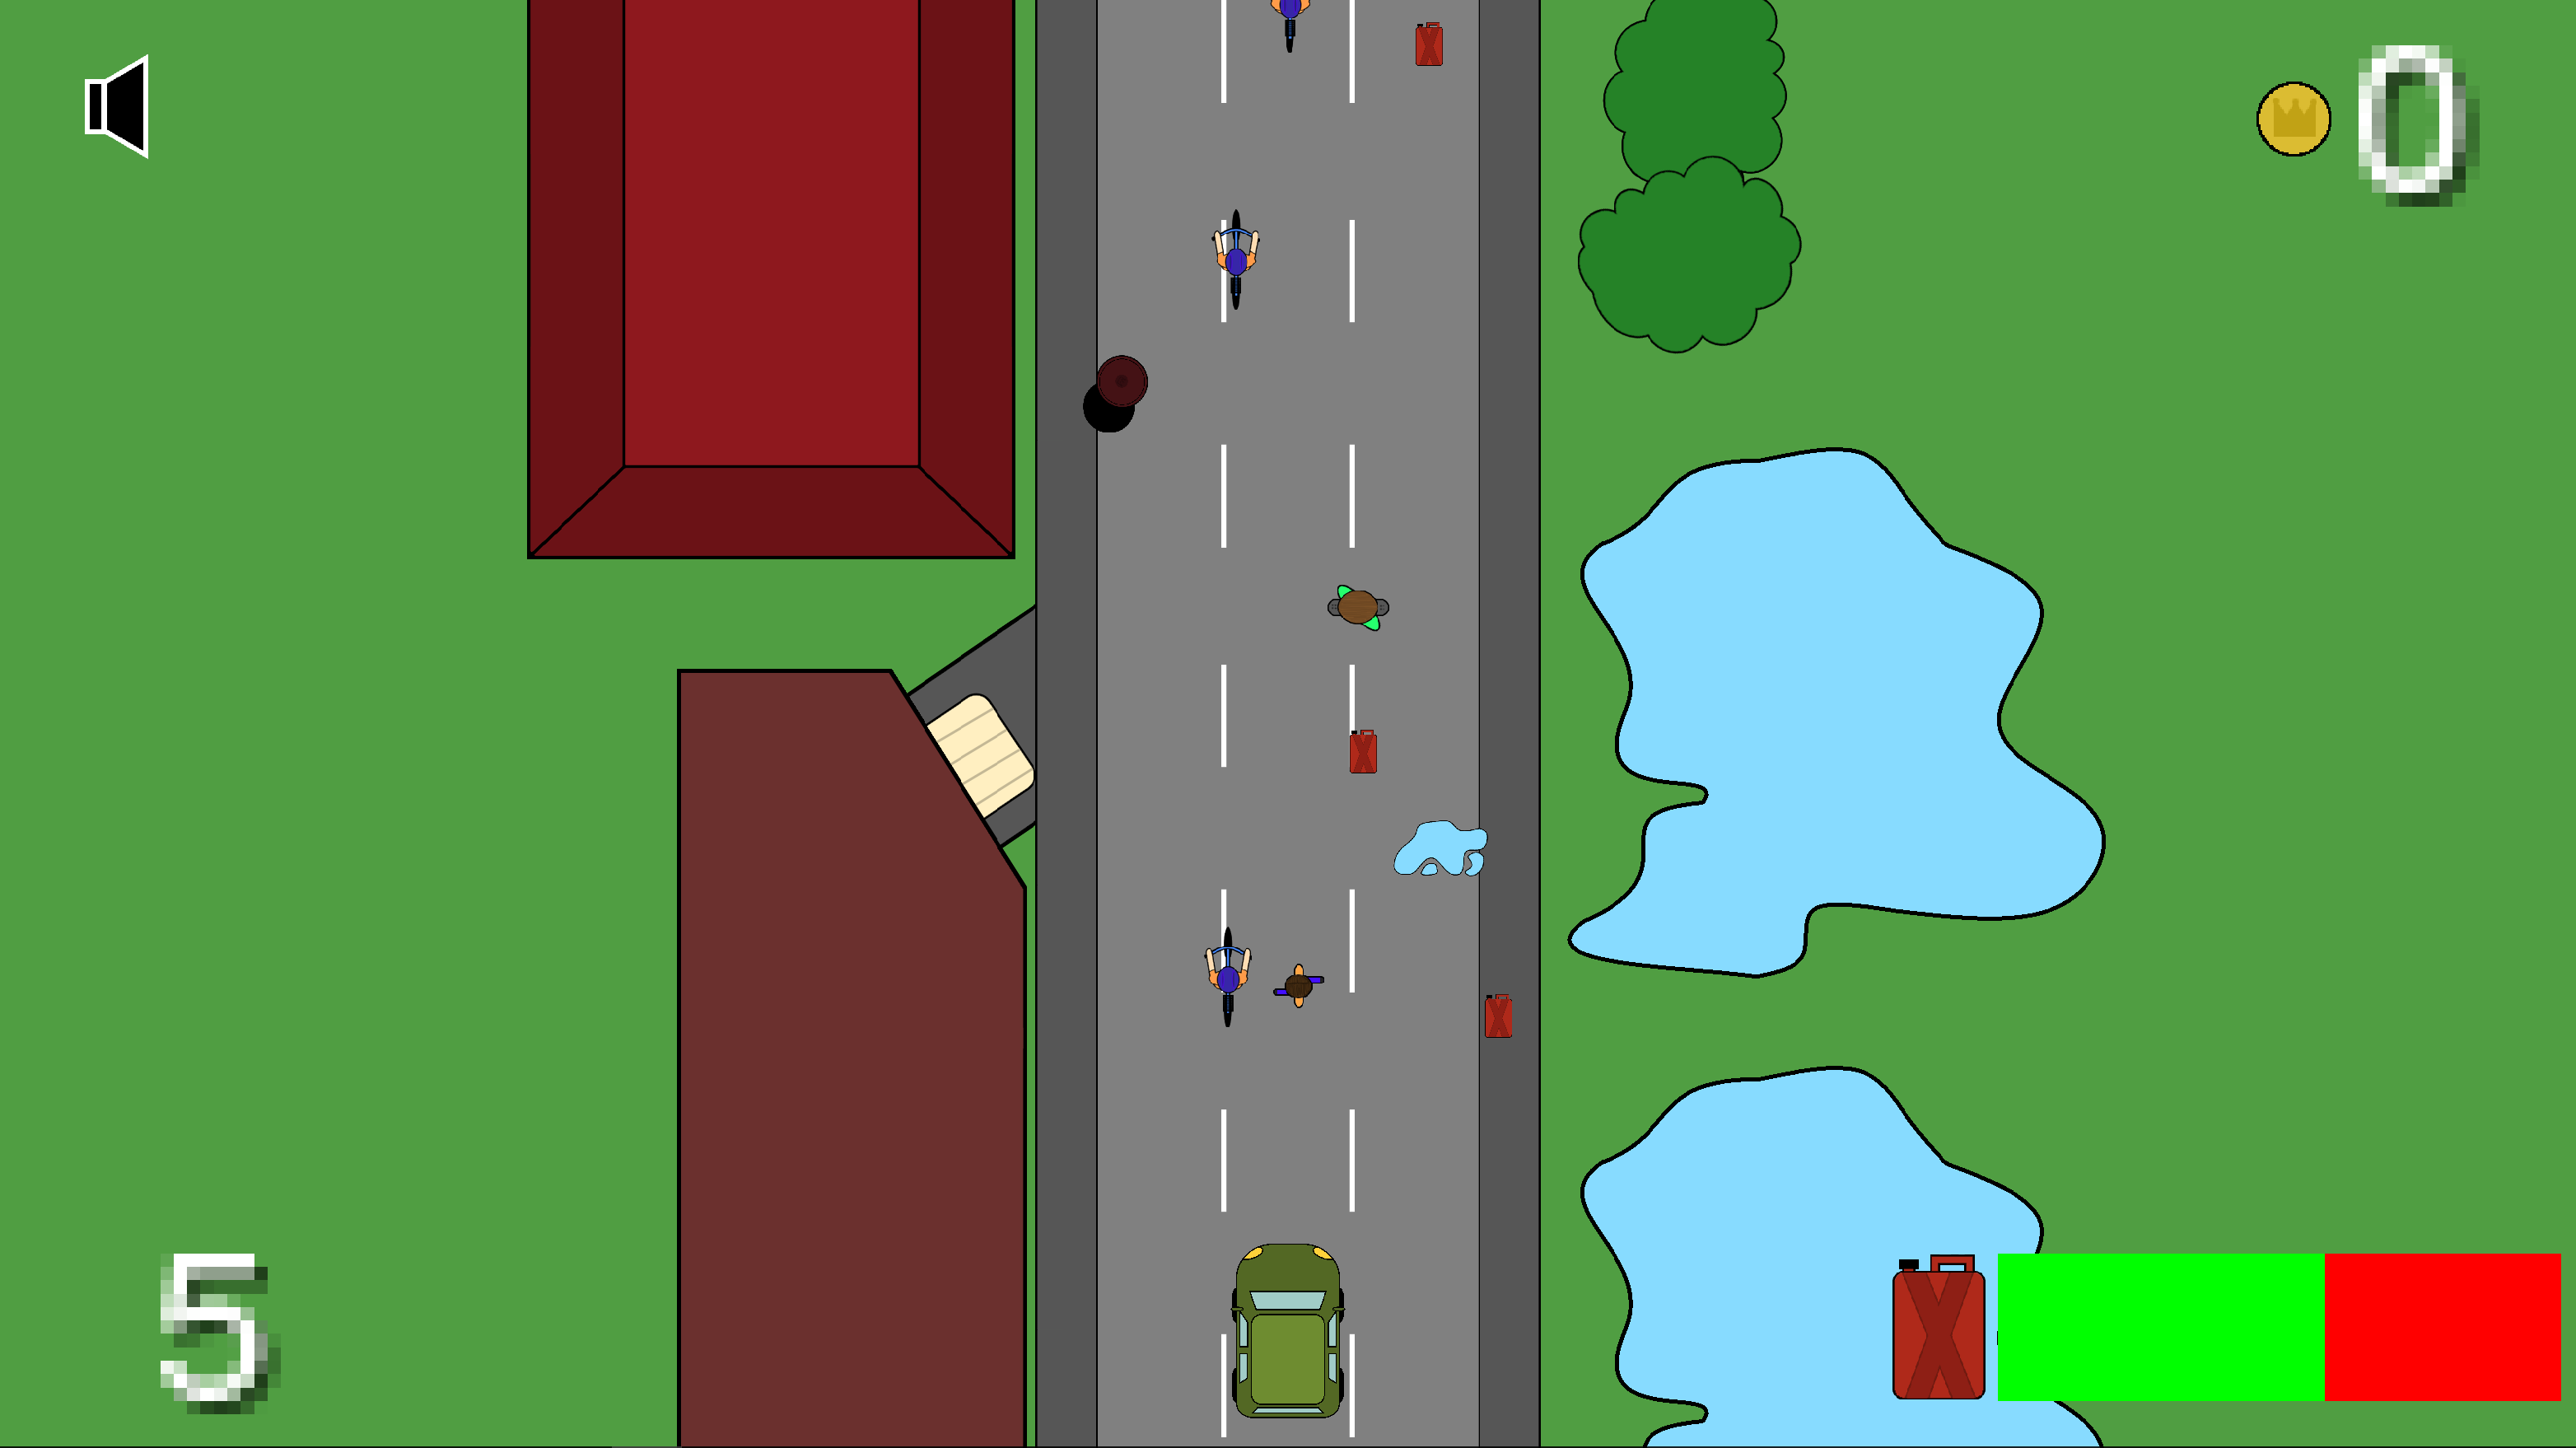
\includegraphics[width=1.00\textwidth]{images/game.PNG}
		\caption{Gameplay.}
	\end{center}\end{figure}

	\begin{figure}\begin{center}
		
\includegraphics[width=1.00\textwidth]{images/pause.PNG}
		\caption{Pausemeny.}
	\end{center}\end{figure}

	\begin{figure}\begin{center}
		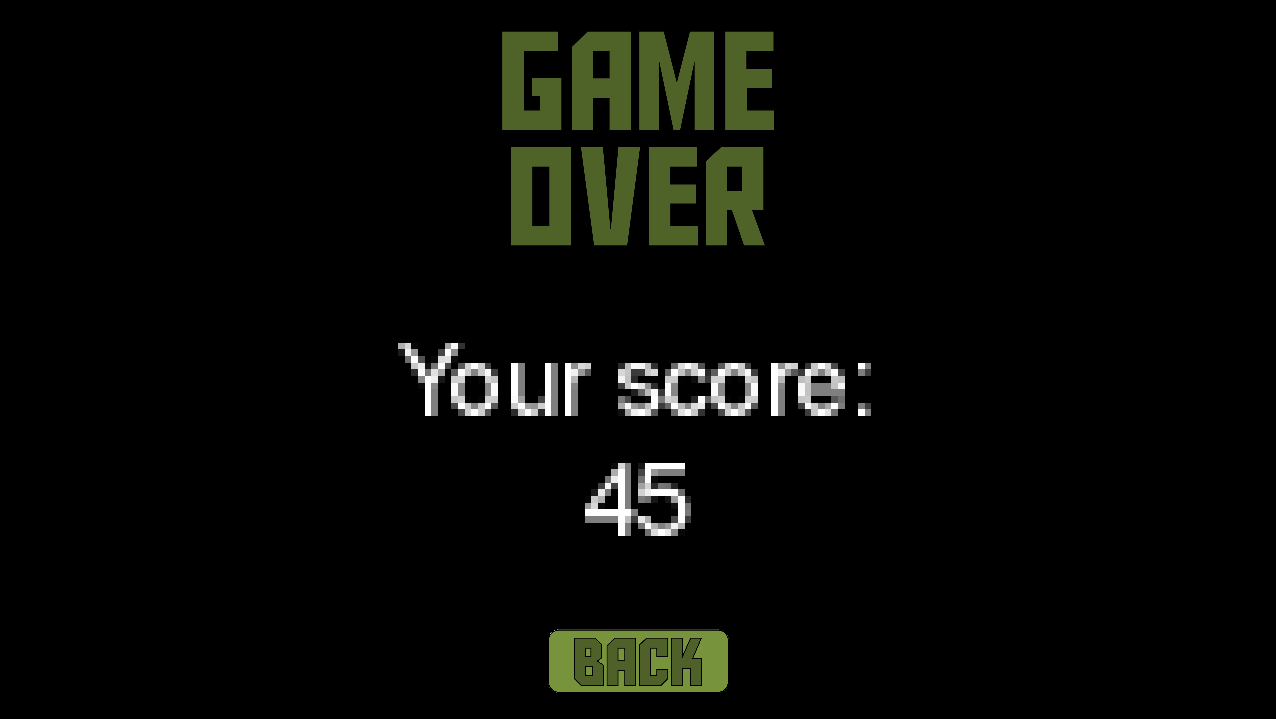
\includegraphics[width=1.00\textwidth]{images/gameover.PNG}
		\caption{Game over-meny.}
	\end{center}\end{figure}


\end{document}